\chapter{Spherical}
\label{sec:spherical}
\section{Spherical Potentials}

\subsection{Plummer}

The plumer density profile is one of the simplest models which describes
a constant density near the center and falls at large radius.

\begin{equation}
\Phi_P(r) = - \frac{GM}{\sqrt{r^2+a^2}}
\end{equation}


Where $a$ is call the scale length. The scale length set the length $a$ in which the mayority of the density is enclosed. Note
that if $a$ is cero the plummer potential would be exactly as the potential of a point mass.
In the other hand if $a$ goes to infinity the potential is represents a very extended mass source.
In other words the scale length set up the size of the volume in which the mass $M$ is enclosed.

Making use of the Poisson's equation one can derive the density from the potential and vice versa.

\begin{equation}
\nabla ^2 \Phi_P(r) = 4 \pi G \rho_P(r) = \frac{1}{r^2}\frac{d}{dr} \left (  r^2 \frac{d\Phi_P(r)}{dr} \right)
\end{equation}

\begin{equation}
\rho_P (r) = \frac{3M}{4\pi a^3} (1 + \frac{r^2}{a^2})^{-5/2}
\end{equation}


The enclosed mass can be derived from the density by integrating over a volume or radius r.

\begin{equation}
M_P(<r) = 4 \pi \int_0^r r'^2\frac{3M}{4\pi a^3} (1 + \frac{r'^2}{a^2})^{-5/2} dr' = \frac{3M}{a^3} \left( \frac{a^4 r^3 \sqrt{r^2/a^2 + 1}}{3(r^2 + a^2)^2}  \right)
\end{equation}

Making some algebra the total mass enclosed in radius $r$ is 
given by:

\begin{equation}
M_P(<r) = M \frac{r^3}{(a^2+r^2)^{3/2}}
\end{equation}

The cirular velocity can be derived from the total enclosed mass
as follows:

%begin{equation}
%_g = \frac{GmM}{r^2} = ma_c = m \frac{v_c^2}{r}
%end{equation}

\begin{equation}
v_c = \sqrt{\frac{GM(<r)}{r}}
\end{equation}

\begin{equation}
v_c = \sqrt{GM\left(\frac{r^2}{( r^2+a^2 ) ^{3/2}}\right)}
\end{equation}


Finally the acceleration can be derived using:

\begin{equation}
a = - \nabla \Phi 
\end{equation}

\begin{equation}
a = - \dfrac{GMr}{(r^2 + a^2)^{3/2}} 
\end{equation}

All this quantities are plotted in Fig.\ref{fig:plummer}.

\begin{figure}[H]
\centering
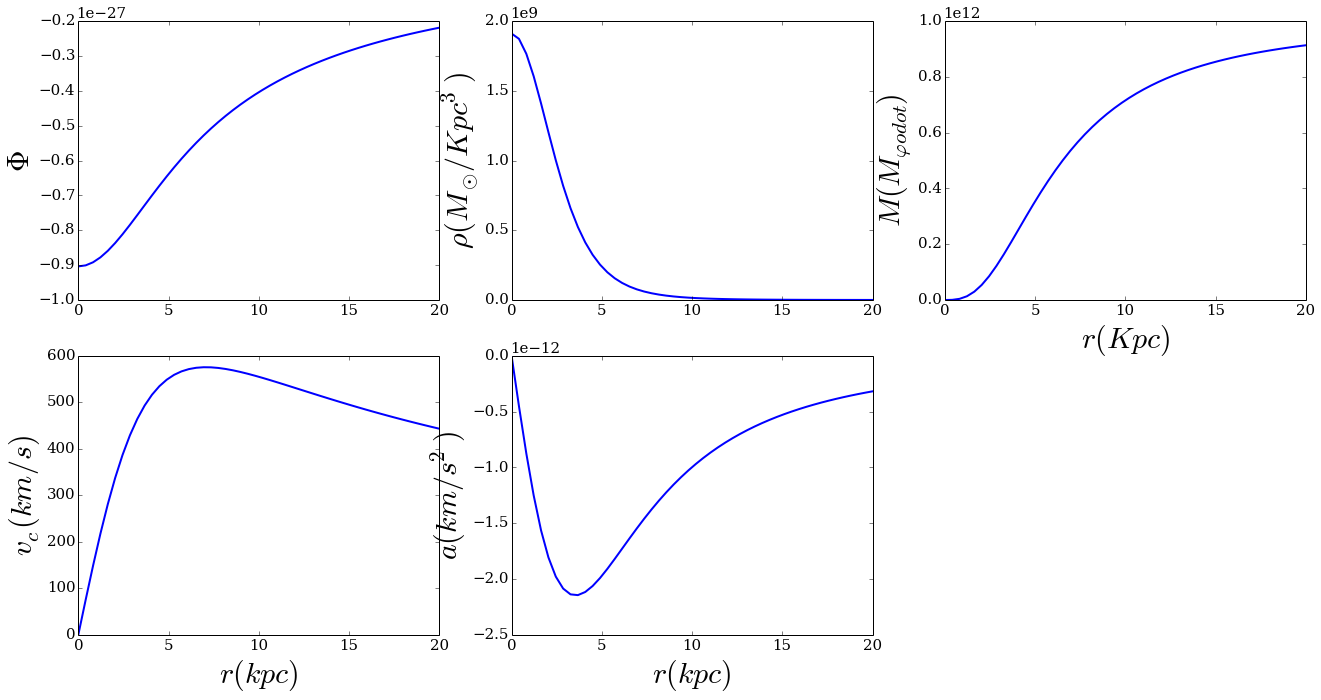
\includegraphics[scale=0.35]{../figures/plummer.png}
\label{fig:plummer}
\end{figure}

\ref{fig:plummer}

\subsection{Hernquist profile}

The Hernquist profile is derived in such a way that it follows the

\begin{equation}
\rho_{Hernquist}(r) =  \frac{M}{2\pi} \frac{a}{r(r+a)^3}
\end{equation}

\begin{equation}
M_{Hernquist}(<r) = 2aM \int \frac{r}{(r+a)^3}dr
\end{equation}

\begin{equation}
M_{Hernquist}(<r) = M \frac{r^2}{(r+a)^2}
\end{equation}

\begin{equation}
\Phi = - \frac{GM}{r+a}
\end{equation}

\begin{equation}
v_c(r) = GM \frac{r}{(r+a)^2}
\end{equation}

\begin{equation}
a = - \dfrac{GM}{(r+a)^2}
\end{equation}


\begin{figure}[H]
\centering
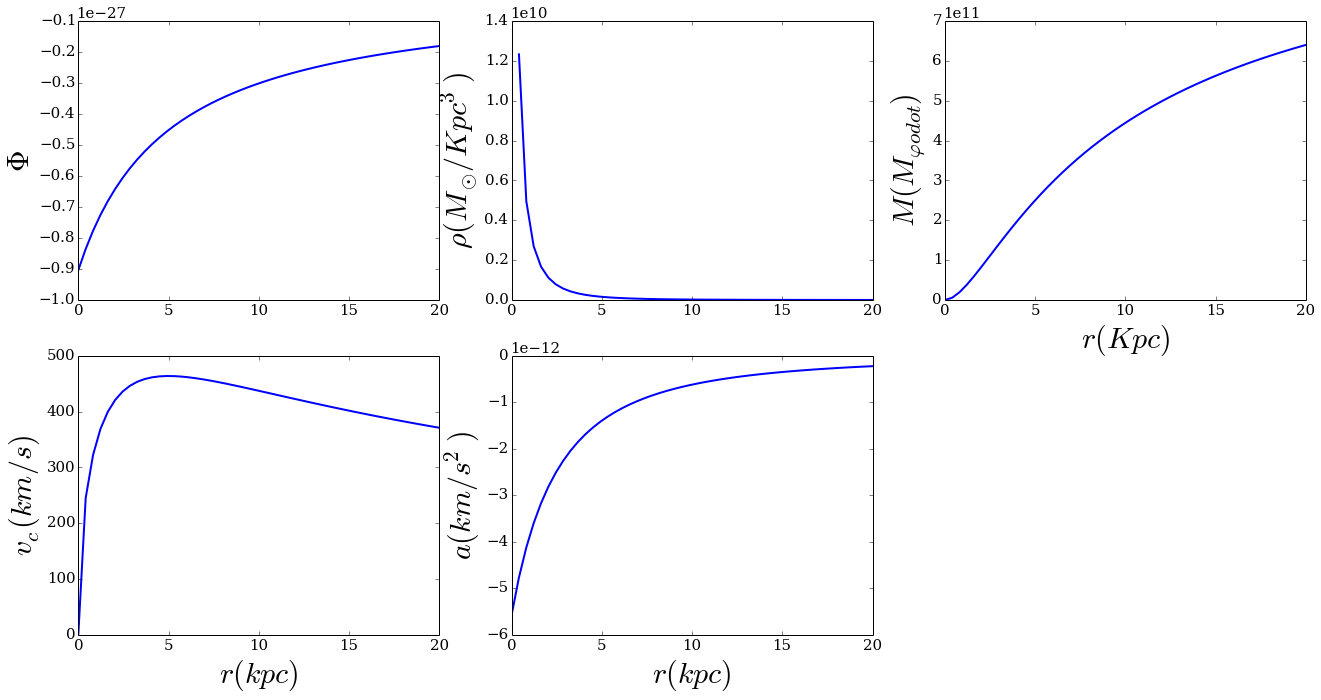
\includegraphics[scale=0.35]{../figures/hernquist.png}
\end{figure}



\subsection{Singular Isothermal Sphere}

The Singular Isothermal Sphere (\textbf{SIS}) describes a system in which the particles follow
a Maxwellian density distribution. With this distribution and the Poisson equation the follow
density profiles could be derived.


\begin{equation}
\rho_{iso}(r) = \dfrac{\sigma ^2}{2\pi G (r^2+a^2)}
\end{equation}

Following the same procedure as with the previuos profiles we find $M, \Phi$  and $v_c$.

\begin{equation}
M_{iso}(<r) = \dfrac{2 \sigma (r+a)}{G}
\end{equation}

\begin{equation}
\Phi_{iso}(r) = 2 \sigma^2 ln(r+a)  + const.
\end{equation}

\begin{equation}\label{eq:SISv}
v_c(r) = \sqrt{2}\sigma
\end{equation}

\begin{equation}
a = - \dfrac{v^2}{(r+a)}
\end{equation}

This profile is quite different to the previous ones due to the fact that here the input is
the velocity instead of the total Mass.

\begin{figure}[H]
\centering
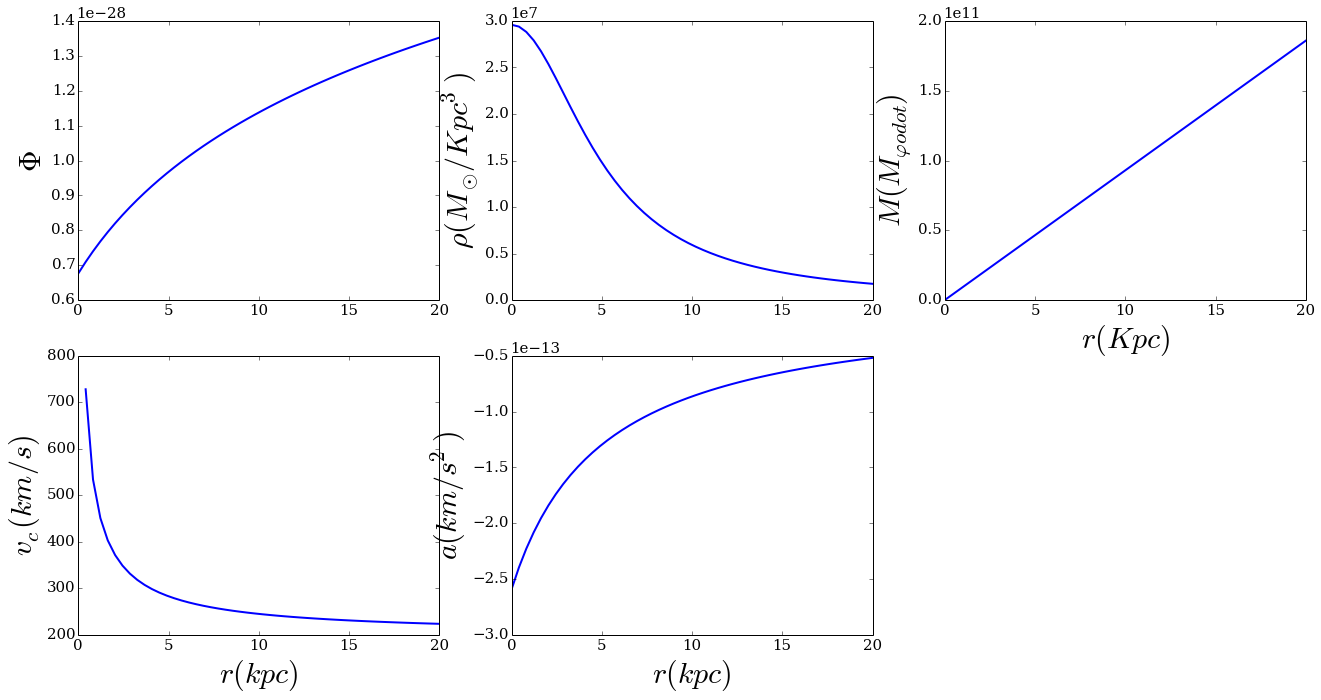
\includegraphics[scale=0.35]{../figures/sis.png}
\end{figure}




\subsection{NFW}


\begin{equation}\label{eq:rhoNFW}
<<<<<<< HEAD
\rho_{NFW}(r) = \dfrac{M_{vir}}{2\pi a^3(r/a) (1 + r/a)^2}
=======
\rho_{NFW}(r) = \dfrac{\rho_s}{(r/a) (1 + r/a)^2}
>>>>>>> 596c3fa464a11f4553321248523034904bcc94ff
\end{equation}


\begin{equation}\label{eq:MNFW}
M_{NFW}(r) =  M_{vir}  f(x) / f(c_{vir})
\end{equation}

Where $x = r/a$, is useful to define the function $f(x)$ as:

\begin{equation}
f(x) = ln(1 + x) - \frac{x}{1 + x} 
\end{equation}

Then \ref{eq:MNFW} can be expresed as:

\begin{equation}\label{eq:M2NFW}
M_{NFW} = 4 \pi \rho_s a^3 f(x) = M_{vir}f(x)/f(c_{vir})
\end{equation}

\begin{equation}\label{PhiNFW}
\Phi_{NFW} = -4\pi G M \frac{ln(1 + r/a)}{r}
\end{equation}

\begin{equation}\label{eq:cnfwz0}
c(M_{vir}) = 9.60  \left( \frac{M_{vir}}{10^{12}h^{-1}M_{\odot}} \right)^{-0.075}
\end{equation}



\begin{equation}\label{vcNFW}
v_c(r) = \sqrt{\left(\dfrac{M(r)G}{r}\right)} = \sqrt{\left( \dfrac{G M_{vir}  f(x) / f(c_{vir})}{r} \right)}
\end{equation}


\begin{figure}[H]
\centering
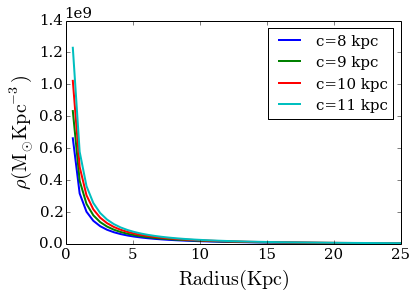
\includegraphics[scale=0.7]{../figures/NFW_density.png}
\end{figure}

\begin{figure}[H]
\centering
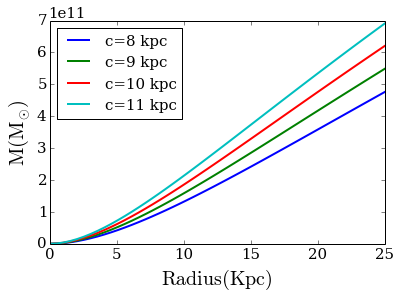
\includegraphics[scale=0.7]{../figures/NFW_mass.png}
\end{figure}

\begin{figure}[H]
\centering
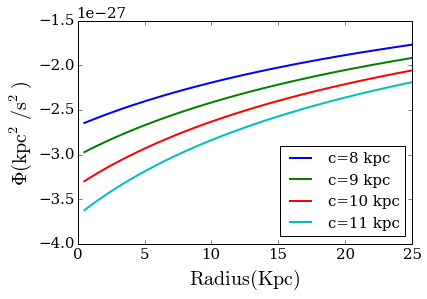
\includegraphics[scale=0.7]{../figures/NFW_potential.png}
\end{figure}

\begin{figure}[H]
\centering
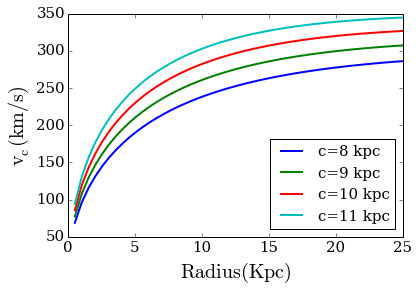
\includegraphics[scale=0.7]{../figures/NFW_vc.png}
\end{figure}



\section{Conversion from NFW to the Hernquist profile}

The average density of the NFW distribution can be expressed as:

\begin{equation}
\bar \rho_{NFW}(r) = \dfrac{3M_{NFW}(r)}{4 \pi r^3} 
\end{equation}

And with eq.\ref{eq:M2NFW} the $\bar{\rho_{NFW}(r)}$ takes de form:

\begin{equation}
\bar \rho_{NFW}(r) = 3 \rho_a \left( \dfrac{a}{r} \right)^{3}  f(x)
\end{equation}

Now if we want to find the relationship betwee $r_{200}$ and $r_{vir}$
for the NFW profile we have to apply eq\ref{eq:q}.

\begin{equation}
q = \dfrac{3 \rho_a \dfrac{a}{r_{200}} f(c_{200})}{3 \rho_a \dfrac{a}{r_{vir}}f(c)} = \dfrac{c_{200}^{3}f(c_{200})}{c_{vir^3}f(c_{vir})}
\end{equation}


\begin{equation}\label{eq:c200cvir}
\dfrac{c_{200}}{c_{vir}} = \left( \dfrac{f(c_{200})}{qf(c_{vir})} \right)^{1/3}
\end{equation}

For $c_{vir} = 10$ this function is shown in Fig.\ref{fig:c200cvir}, where
$y = \dfrac{c_{200}}{c_{vir}} - \left( \dfrac{f(c_{200})}{qf(c_{vir})} \right)^{1/3}$

\begin{figure}[H]\label{fig:c200cvir}
\centering
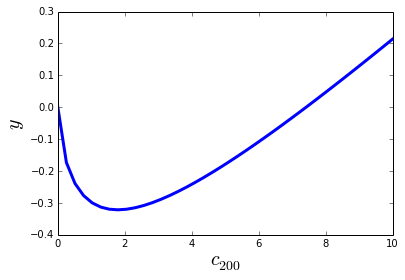
\includegraphics[scale=0.7]{../figures/c200cvir.png}
\end{figure}

Note that the solution of Eq.\ref{eq:c200cvir} is when $y=0$, one
solution is $c_{200}=0$ but this is not of particular interest for us.

The other solution is computed analytically using the bisection algorithm.
$c_{200} = 7.4$

In order to seek the equivalence between the NFW and the Hernquist profile,
We have to match the same enclosed mass of both profiles at a given radius.
To his end we have to find $M_H$ in terms of $r_s$.

\begin{equation}
M_H(r) = M_{NFW}(r)
\end{equation}

\begin{equation}
\frac{M_H r^2}{a^2 + r^2} = 4 \pi \rho_s r_s^3 \left[ Ln(1 + x) - \frac{x}{1+x}  \right]
\end{equation}

In the limit $r \rightarrow 0$

\begin{equation}
M_H = \dfrac{4 \pi \rho_s r_s^3 a^2}{r^2} \left[ (x - \dfrac{x^2}{2}) - x  \right]
\end{equation}

\begin{equation}
M_H = 4 \pi \rho_s r_s^3 \dfrac{a^2}{r^2} \left(  - \dfrac{r^2}{2r_s^2} \right)
\end{equation}

\begin{equation}
M_H = 2 \pi r_s a^2
\end{equation}

With this relation is possible now to match both profiles at a given radius $\tilde{r}$

\begin{equation}
M_H(\tilde{r}) = M_{NFW}(\tilde{r}) 
\end{equation}

\begin{equation}
2 \pi \rho_s a^2 r_s \dfrac{\tilde{r}^2}{a^2} \dfrac{1}{\left( 1 + \dfrac{\tilde{r}}{a}\right)^2} = 4 \pi \rho_s r_s^3 \left( Ln \left(1 + \dfrac{\tilde{r}}{r_s} \right)  - \dfrac{\tilde{r}}{\tilde{r} + r_s} \right)
\end{equation}

\begin{equation}
\dfrac{\tilde{r}^2 a^2}{(a + \tilde{r})^2} = 2 r_s^2 \left( Ln \left (1 +  \dfrac{\tilde{r}}{r_s} \right)  - \dfrac{\tilde{r}}{\tilde{r} + r_s}   \right)
\end{equation}


\begin{equation}
\dfrac{\tilde{r}^2 a^2}{(a + \tilde{r})^2} = 2 r_s^2 f(\tilde{x})
\end{equation}

\begin{equation}
\left( \frac{a}{r_s} \right)^2 = \dfrac{2}{\tilde{r}^2} (a + \tilde{r})^2 f(\tilde{x})
\end{equation}




\begin{equation}
\dfrac{a}{r_s} = \dfrac{[2 f(\tilde{x})]^{1/2}}{\tilde{r}} (a + \tilde{r})
\end{equation}

\begin{equation}
\left( \dfrac{a}{r_s} \right) \left( 1 -  \dfrac{[2 f(\tilde{x})]^{1/2}}{\tilde{x}} \right) = [2 f(\tilde{x})]^{1/2} 
\end{equation}

\begin{equation}
\dfrac{a}{r_s} = \dfrac{[2 f(\tilde{x})]^{1/2}}{ \left( 1 -  \dfrac{[2 f(\tilde{x})]^{1/2}}{\tilde{x}} \right)}
\end{equation}

\begin{equation}
\dfrac{a}{r_s} = \dfrac{[2 f(\tilde{x})]^{1/2} \tilde{x}}{\tilde{x} - (2f(\tilde{x})^{1/2})} = \dfrac{1}{\left(  [2 f(\tilde{x})]^{-1/2} - \dfrac{1}{\tilde{x}}  \right)}
\end{equation}

Finally the ratio of the enclosed mass of the Hernquist and the NFW profiles is:

\begin{equation}
\dfrac{M_H}{M_{vir}} = \dfrac{2 \pi \rho_s a^2 r_s}{4 \pi \rho_s r_s^3 f(c_{vir})} = \dfrac{1}{2 f(c_{vir})}  \left( \dfrac{a}{r_s}\right)^2
\end{equation}


